\documentclass{../tuda-exercise}

% Title information
\version{20. November 2021}
\sheetnumber{10}

\begin{document}

  \maketitle

  \begin{task}[credit = \stars{0}{3}]{Theoriefragen}
    Welche der folgenden Aussagen ist wahr?
    \begin{enumerate}
      [label = (\Alph*)]
      \item Streams können aus Listen und Arrays erzeugt werden.
      \item Man kann nur mit Iteratoren über die einzelnen Elemente in einem Stream gehen.
      \item Ein Objekt der Klasse \inlinejava{Path} verwaltet den Pfadnamen einer Datei oder
      eines Verzeichnisses oder eines anderen Objektes, das im jeweiligen Dateisystem über einen
      Pfadnamen ansprechbar ist.
      \item Streams können in sich Daten speichern.
      \item Byteweiser Zugriff ist nur dann sinnvoll, wenn eine Datei nur Text und keine Bilder,
      Audio- oder Videodateien enthält, da bei einem Text die Bytes leichter gelesen werden können.
      \item \inlinejava{Runnable} ist ein Functional Interface. Die funktionale Methode heißt
      \inlinejava{run}, hat keine Parameter und ist \inlinejava{void}.
      \item Einzelne Threads können nicht terminiert werden, sie enden alle mit dem Ende des
      Gesamtprogramms.
      \item Eine Parallelisierung mit Threads verkürzt immer die Laufzeit eines Programms.
      \item Wann immer auf einen Button geklickt wird, wird Methode \inlinejava{actionPerformed}
      jedes bei diesem Button registrierten Listeners aufgerufen.
      \item Für jede Art von Listener gibt es eine eigene Registrierungsmethode.
      \item Die Klasse \inlinejava{Canvas} bietet eine unbegrenzte Zeichenfläche in einem Fenster.
    \end{enumerate}

    \clearpagesolution

    \begin{solution}
      \begin{enumerate}
        [label = (\Alph*)]
        \item Wahr. Jede Collection besitzt die Methode
        \href{https://docs.oracle.com/en/java/javase/11/docs/api/java.base/java/util/Collection.html#stream()}
        {\inlinejava{stream()}}. Da das Interface \inlinejava{List} \inlinejava{Collection}
        erweitert, kann sie ebenfalls auf die Methode zugreifen. Um einen Stream aus einem Array
        zu erzeugen, gibt es folgende Möglichkeiten:
        \begin{itemize}
          \item \href{https://docs.oracle.com/en/java/javase/11/docs/api/java.base/java/util/Arrays.html#stream(T[])}
          {\inlinejava{Arrays.stream(T[] array)}}
          \item \href{https://docs.oracle.com/en/java/javase/11/docs/api/java.base/java/util/stream/Stream.html#of(T...)}
          {\inlinejava{Stream.of(T... values)}}
          \item \inlinejava{Arrays.stream(...)} gibt es ebenfalls für primitive Datentypen, außer für
          \inlinejava{byte} und \inlinejava{char}.
        \end{itemize}
        \item Wahr, da Streams nicht mit einem Index arbeiten und man dadurch nicht auf ein
        einzelnes Element im Stream zugreifen kann.
        \item Wahr. Außerdem muss es zum Pfadnamen in einem Path-Objekt keine Datei o.ä. im
        Dateisystem geben (sonst könnte man damit ja auch keine neue Datei erzeugen).
        \item Inkorrekt, Streams können zwar Daten in sich speichern, jedoch sind diese zur
        Bearbeitung der Daten gedacht und nicht zur permanenten Speicherung der Daten.
        \item Inkorrekt, da byteweiser Zugriff besser für Bild, Video oder Audiodaten geeignet
        ist. Generell sollte man für Texte \textbf{keine} Bytedaten verwenden.
        \item Wahr, es existiert ein Functional-Interface namens \inlinejava{Runnable} mit der
        erwähnten Methode (Package \inlinejava{java.lang}.
        \item Inkorrekt, man kann einzelne Threads zu jeder Zeit stoppen ohne auf das Ende des
        Gesamtprogramms zu warten.
        \item Inkorrekt, da Threads auch für mehr Laufzeit sorgen können, da sie selbst auch
        Laufzeit zu einem Programm hinzufügen. Also, wenn man zu viele Threads verwendet, kann
        das Programm langsamer als das ursprüngliche Programm ohne Threads werden.
        \item Wahr, da ein Button immer alle zu sich hinzugefügten Listener aufruft.
        \item Wahr.
        \item Wahr, jedoch wird das Canvas nur innerhalb des Fensters angezeigt.
      \end{enumerate}

      \begin{note}[title=Information:]
        Die Abbildung \ref{fig:V1_Information} stellt eine beispielhafte Visualisierung von einem
        \href{https://docs.oracle.com/en/java/javase/11/docs/api/java.base/java/util/stream/Stream.html}{Stream} dar
        und hilft Ihnen vielleicht Streams besser zu verstehen.

        \begin{figure}[H]
          \centering
          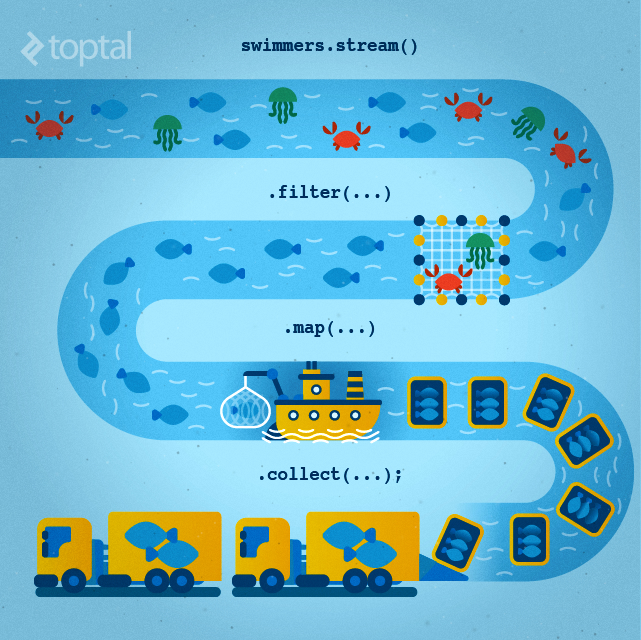
\includegraphics[width=.45\linewidth]{graphics/stream_visual.png}
          \caption{Quelle \url{https://www.exclamationlabs.com/blog/refactoring-for-java-8-streams/}}
          \label{fig:V1_Information}
        \end{figure}
      \end{note}
    \end{solution}
  \end{task}

  \clearpage

  \begin{task}[credit = \stars{1}{3}]{Vereinfachung mittels Lambda-Ausdrücken}
    Gegeben sei nachstehender Java-Code. In diesem wird aus einer Liste von Zahlen der
    Durchschnittswert aller \textit{positiven geraden Zahlen} berechnet, in einer Variablen
    gespeichert und zurückgegeben.

    \lstinputlisting[style = Java]{codes/V2_Task.java}

    \begin{enumerate}
      \item Nutzen Sie Streams und Lambda-Ausdrücke um den Code zu verkürzen.
      \item Beide Implementierungen – die \enquote{normale} und die \inlinejava{Stream}-Variante
      – weisen eine konzeptionelle Unsauberkeit auf. Bei beiden kann es zum Auftreten einer
      \inlinejava{Exception} kommen.
      \begin{enumerate}
        [label = (\alph*)]
        \item An welcher Stelle kann es bei der \enquote{normale} Implementierung zu einer
        \inlinejava{Exception} kommen? Um welche handelt es sich?
        \item An welcher Stelle kann es bei der Implementierung mittels Streams zu einer
        \inlinejava{Exception} kommen? Um welche handelt es sich?
      \end{enumerate}
      \item Modifizieren Sie den Code entsprechend, dass die Exceptions aus Teilaufgabe 2 gar
      nicht mehr auftreten können, sondern die Methode für alle übergebenen Arrays fehlerfrei
      durchläuft.
    \end{enumerate}

    \clearpagesolution

    \begin{solution}
      \begin{enumerate}
        \item\hfill
        \lstinputlisting[style = Java]{codes/V2_Solution.java}
        \item
        \begin{enumerate}
          [label = (\alph*)]
          \item Eine \inlinejava{NullPointerException} wird geworfen, falls der übergebene
          Parameter gleich \inlinejava{null} ist. Ansonsten gibt es eine weitere konzeptionelle
          Unsauberkeit: Wenn der Wert von \inlinejava{count} 0 ist, würde die Methode zwar keine
          \inlinejava{Exception} werfen, jedoch wird
          \href{https://docs.oracle.com/en/java/javase/11/docs/api/java.base/java/lang/Double.html#NaN}
          {\inlinejava{Double.NaN}} zurückgegeben.
          \item Wie bei der \enquote{normalen} Implementierung wird hier ebenfalls eine
          \inlinejava{NullPointerException} geworfen. Des weiteren weist die Implementierung eine
          weitere konzeptionelle Unsauberkeit auf: Falls die nach dem Filter der Stream leer ist,
          gibt der Aufruf von \inlinejava{average()} einen leeren
          \href{https://docs.oracle.com/en/java/javase/11/docs/api/java.base/java/util/OptionalDouble.html}
          {\inlinejava{OptionalDouble}} zurück. Wenn wir nun \inlinejava{getAsDouble()} aufrufen,
          wird eine \inlinejava{NoSuchElementException} geworfen, da das
          \inlinejava{OptionalDouble} keine Werte enthält.
        \end{enumerate}
        \item Man kann die Probleme bei der Stream-Variante beheben, indem man statt
        \inlinejava{getAsDouble()}
        \href{https://docs.oracle.com/en/java/javase/11/docs/api/java.base/java/util/OptionalDouble.html#orElse(double)}
        {\inlinejava{orElse(0)}} aufruft, wodurch entweder der vorhandene Wert des
        \inlinejava{OptionalDouble} oder, wenn kein Wert vorhanden ist, 0 zurückgegeben wird. In
        der \enquote{normalen} Variante kann man die Probleme beheben, indem man vor oder in
        Zeile 9 auf \inlinejava{count} \(> 0\) testet und bei  \inlinejava{count} \(\leq 0\)
        einen Standardwert (z.B: \(0\)) zurückgibt. Um die \inlinejava{NullPointerException} in
        beiden Implementierung zu umgehen, reicht zu Beginn eine Abfrage, ob das Array gleich
        \inlinejava{null} ist.
      \end{enumerate}
    \end{solution}
  \end{task}

  \clearpagesolution

  \begin{task}[credit = \stars{1}{3}]{Mein eigenes kleines Fenster}
    Implementieren Sie ein kleines Programm mit einer GUI, welche genauso aussieht wie in der
    nachfolgenden Abbildung:

    \begin{figure}[h]
      \centering
      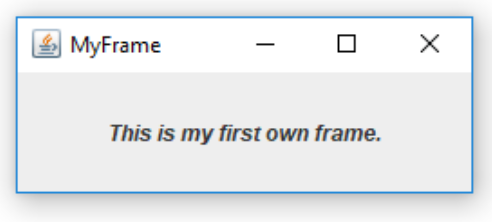
\includegraphics[width = 0.5\textwidth]{graphics/V3_Task.png}
    \end{figure}

    \begin{solution}
      \lstinputlisting[style = Java]{codes/V3_Solution.java}
    \end{solution}
  \end{task}

  \clearpagesolution

  \begin{task}[credit = \stars{2}{3}]{Innere Klassen und Scope}
    Betrachten Sie den untenstehenden Java-Code, welcher eine innere Klasse
    \inlinejava{InnerClass} enthält. In dieser wiederum ist eine Methode definiert, die einen
    Lambda-Ausdruck enthält, dessen Operation mit der Methode \inlinejava{accept} des Interface
    \inlinejava{Consumer} aufgerufen wird.

    \lstinputlisting[style = Java]{codes/V4_Task.java}

    Welche Ausgabe wird bei der Ausführung des Codes auf der Konsole ausgegeben? Überlegen Sie
    sich die Antworten ohne die Nutzung eines Compilers!

    \begin{solution}
      \begin{itemize}
        \item \inlinejava{x = 123}
        \item \inlinejava{y = 123}
        \item \inlinejava{this.x = 11}
        \item \inlinejava{LambdaScope.this.x = 0}
        \item \inlinejava{z = 55}
      \end{itemize}
    \end{solution}
  \end{task}

  \begin{task}[credit = \stars{2}{3}]{Zeilen nummerieren}
    Implementieren Sie die Methode \inlinejava{void insertRowNumbers(String path)}, welche den
    Pfad einer Text-Datei als \inlinejava{String} übergeben bekommt. Die Methode soll den Text
    der Datei Zeile für Zeile einlesen. Beginnend ab der ersten Zeile soll dann in jeder zweiten
    Zeile nun die Zeilennummer eingefügt werden. War die alte Text-Datei folgendermaßen
    aufgebaut: \code{\textcolor{stringcolor}{"'Row1 \(\backslash\)n Row2"'}} so soll die neue
    Text-Datei so aussehen: \code{\textcolor{stringcolor}{"'1 Row1 \(\backslash\)n 2 Row2"'}}. Dabei steht
    \code{\textcolor{stringcolor}{"'\(\backslash\)n"'}} für einen Zeilenumbruch.

    \begin{solution}
      \lstinputlisting[style = Java]{codes/V5_Solution.java}
    \end{solution}
  \end{task}

  \clearpage

  \begin{task}[credit = \stars{3}{3}]{Bäckerei gesucht}
    Sie planen eine Party und benötigen eine Menge Brötchen dafür. Sie suchen nun den Bäcker in
    Ihrer Umgebung, der Ihnen die günstigsten Brötchen verkaufen kann. Dafür gibt es Objekte des
    Typs \inlinejava{Bakery}, welche zum einen zwei \inlinejava{public double}-Attribute
    \inlinejava{distance} (gibt die Distanz zu Ihnen in km an) und \inlinejava{price} (gibt den
    Preis pro Brötchen an) besitzt. Außerdem gibt es Objekte des Typs \inlinejava{BakeryOffer},
    welche ebenfalls zwei \inlinejava{public}-Attribute \inlinejava{bakery} vom Typ
    \inlinejava{Bakery} und \inlinejava{totalPrice} vom Typ \inlinejava{double} besitzt. Der
    Konstruktor der Klasse sieht folgendermaßen aus:

    \lstinputlisting[style = Java]{codes/V6_Task.java}

    Implementieren Sie nun eine \inlinejava{public}-Methode vom Rückgabetyp
    \inlinejava{List<BakeryOffer>} mit dem
    Methodenkopf:

    \begin{center}
      \inlinejava{sortedBakeryOffers(Collection<Bakery> bakeries, double maxDistance)}
    \end{center}

    Die Methode erhält eine Sammlung von Bäckereien und die maximale Distanz zu einer solchen.
    Zurückgeliefert werden soll eine nach Gesamtpreis aufsteigend sortierte Liste mit Angeboten
    des Typs \inlinejava{BakeryOffer}. Bäckereien, die weiter als die übergebene maximale Distanz
    entfernt sind, sollen von der Betrachtung ausgeschlossen werden.

    \begin{solution}
      \lstinputlisting[style = Java]{codes/V6_Solution.java}
    \end{solution}
  \end{task}

  \clearpagesolution

  \begin{task}[credit = \stars{3}{3}]{Zähler}
    Implementieren Sie ein kleines Programm mit einer GUI, welche genauso aussieht wie in der
    nachfolgenden Abbildung:

    \begin{figure}[h]
      \centering
      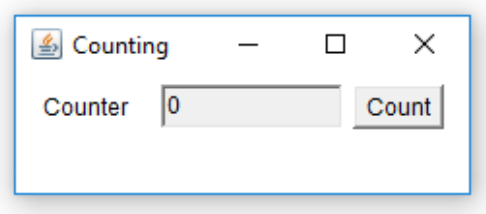
\includegraphics[width = 0.5\textwidth]{graphics/V7_Task.png}
    \end{figure}

    Jedes Mal wenn der \textit{Count}-Button gedrückt wird, soll sich der Wert im Feld um
    \inlinejava{1} erhöhen.

    \br

    \begin{note}[title=Hinweis:, color=tuda-orange]
      Ihr Programm besteht aus drei Komponenten:
      \begin{enumerate}
        \item \inlinejava{java.awt.Label} \code{\textcolor{stringcolor}{"'Counter"'}}
        \item \footnote{\url{http://programmedlessons.org/java5/Notes/chap60/ch60_13.html}}{non-editable}
        \inlinejava{java.awt.TextField}
        \item \inlinejava{java.awt.Button} \code{\textcolor{stringcolor}{"'Count"'}}
      \end{enumerate}
    \end{note}

    \clearpagesolution

    \begin{solution}
      \lstinputlisting[style = Java]{codes/V7_Solution.java}
    \end{solution}
  \end{task}
\end{document}
